\section{Architecture\label{sec:radar.archi}}

This section details \thecontrib's architecture.
It is divided into three main components:
\begin{enumerate*}[label=(\emph{\roman*})]
    \item our cross-evaluation scheme that provides local feedbacks on each participant's contributions~(\Cref{sec:radar.archi.xeval}),
    \item a similarity-based clustering algorithm that groups participants based on evaluations~(\Cref{sec:radar.archi.cluster}), and 
    \item a reputation system that assesses participants' trustworthiness based on their past contributions (\Cref{sec:radar.archi.reput}).
\end{enumerate*}
\Cref{fig:radar.archi} provides an overview of \thecontrib.

\begin{figure}
    \centering
    \scalebox{0.7}{
    \tikzstyle{block}=[draw, minimum size=0.7cm, node distance=2cm, circle, shape=rectangle, minimum width=2.3cm]

\tikzstyle{arrow}=[thick, -latex]
\tikzstyle{darrow}=[latex-latex, thick,]
\tikzstyle{model}=[draw=blue, dashed]
\tikzstyle{eval}=[draw=violet, dotted]
\tikzstyle{cluster}=[draw=orange]
\tikzstyle{weight}=[draw=green, dashdotted]

\begin{tikzpicture}[sloped]
	\node (center) {};
	\node[block, above of=center, node distance=1cm] (training) {Local training};
	\node[block, below of=center, node distance=1cm] (eval) {Evaluation};
	\node[right of=center, node distance=2cm] (sep) {};
	\node[ above of=sep, node distance=2cm] (top) {};
	\node[ below of=sep, node distance=2cm] (bottom) {};
	\node[left of=top] (clients) {Clients};
	\node[right of=top] (server) {Server};
	\node[block, right of=sep, node distance=3cm] (orchestration) {Orchestration};
	\node[block, above right of=orchestration] (clustering) {Clustering};
	\node[block, right of=orchestration, node distance=3cm] (reputation) {Reputation};
	\node[block, below left of=reputation] (agg) {Aggregation};
        \node[ below of=orchestration, node distance=3cm] (legend) {};
        \node[ left of=legend, node distance=3cm] (legend_start) {};
        % \draw (legend) node[anchor=south] {.};
	
        \draw[thick, dashed] (top.north) -- (bottom);

	\node[right of=legend_start, node distance=0.5cm] (legend1) {};
	\node[above of=legend1, node distance=0.6cm] (legend2) {};
	\node[right of=legend1, node distance=2cm] (legend3) {};
	\node[above of=legend3, node distance=0.6cm] (legend4) {};

	\draw[arrow, model] (legend1) -- ++(2cm,0) node [midway, below, sloped] {Models};
	\draw[arrow, eval] (legend2) -- ++(2cm,0) node [midway, below, sloped] {Evaluations};
	\draw[arrow, cluster] (legend3) -- ++(2cm,0) node [midway, below, sloped] {Clusters};
	\draw[arrow, weight] (legend4) -- ++(2cm,0) node [midway, below, sloped] {Weights};
	
	\draw[arrow, eval] (orchestration.north)  |- (clustering.west);
	\draw[arrow, eval] (orchestration.east)  |- (reputation);
	\draw[arrow, cluster] (clustering.south) |- ($(reputation.west)!0.5!(reputation.north west)$);
	\draw[arrow, cluster] (clustering.east)  |-  ++( 2cm, 0) |- (agg.east);
	\draw[darrow, model] (orchestration) |- (agg);
	\draw[arrow, weight] (reputation) |- ($(agg.east)!0.5!(agg.north east)$);
	\draw[darrow, model] ($(training.east)!0.5!(training.south east)$) -- ($(orchestration.west)!0.5!(orchestration.north west)$);
	\draw[arrow, eval] ($(eval.east)!0.2!(eval.north east)$)-- ($(orchestration.west)!0.5!(orchestration.south west)$);
	\draw[arrow, model] ($(orchestration.west)!0.2!(orchestration.south west)$) --  ($(eval.east)!0.5!(eval.north east)$);
\end{tikzpicture}

% \begin{tikzpicture}[sloped]
% 	\node (center) {};
% 	\node[block, above of=center, node distance=1cm] (training) {Local training};
% 	\node[block, below of=center, node distance=1cm] (eval) {Evaluation};
% 	\node[right of=center, node distance=2cm] (sep) {};
% 	\node[ above of=sep, node distance=2cm] (top) {};
% 	\node[ below of=sep, node distance=2cm] (bottom) {};
% 	\node[left of=top] (clients) {Clients};
% 	\node[right of=top] (server) {Server};
% 	\node[block, right of=sep, node distance=3cm] (orchestration) {Orchestration};
% 	\node[block, above right of=orchestration] (clustering) {Clustering};
% 	\node[block, right of=orchestration, node distance=3cm] (reputation) {Reputation};
% 	\node[block, below left of=reputation] (agg) {Aggregation};
% 
% 	\draw[thick, dashed] (top.north) -- (bottom);
% 
% 	\node[below of=bottom, node distance=0.5cm] (legend1) {};
% 	\node[below of=legend1, node distance=0.5cm] (legend2) {};
% 	\node[right of=legend1, node distance=2cm] (legend3) {};
% 	\node[below of=legend3, node distance=0.5cm] (legend4) {};
% 
% 	\draw[arrow, model] (legend1) -- ++(2cm,0) node [midway, below, sloped] {Models};
% 	\draw[arrow, eval] (legend2) -- ++(2cm,0) node [midway, below, sloped] {Evaluations};
% 	\draw[arrow, cluster] (legend3) -- ++(2cm,0) node [midway, below, sloped] {Clusters};
% 	\draw[arrow, weight] (legend4) -- ++(2cm,0) node [midway, below, sloped] {Weights};
% 	
% 	\draw[arrow, eval] (orchestration.north)  |- (clustering.west);
% 	\draw[arrow, eval] (orchestration.east)  |- (reputation);
% 	\draw[arrow, cluster] (clustering.south) |- ($(reputation.west)!0.5!(reputation.north west)$);
% 	\draw[arrow, cluster] (clustering.east)  |-  ++( 2cm, 0) |- (agg.east);
% 	\draw[darrow, model] (orchestration) |- (agg);
% 	\draw[arrow, weight] (reputation) |- ($(agg.east)!0.5!(agg.north east)$);
% 	\draw[darrow, model] ($(training.east)!0.5!(training.south east)$) -- ($(orchestration.west)!0.5!(orchestration.north west)$);
% 	\draw[arrow, eval] ($(eval.east)!0.2!(eval.north east)$)-- ($(orchestration.west)!0.5!(orchestration.south west)$);
% 	\draw[arrow, model] ($(orchestration.west)!0.2!(orchestration.south west)$) --  ($(eval.east)!0.5!(eval.north east)$);
% \end{tikzpicture}
    }
    \caption{\label{fig:radar.archi}\emph{Architecture overview.}}
\end{figure}


\subsection{Assessing Contributions with Cross-Evaluation\label{sec:radar.archi.xeval}}

As highlighted in~\Cref{sec:radar.related}, most related works on poisoning mitigation in \gls{fl} rely on server-side models comparison~\cite{fung_LimitationsFederatedLearning_2020,awan_CONTRADefendingPoisoning_2021}. 
They measure distance between the parameters (for \glspl{dnn}, $n$-dimensional arrays containing the weights and biases of each neuron) using metrics such as cosine similarity~\cite{fung_LimitationsFederatedLearning_2020} or Euclidean distance~\cite{ma_ShieldFLMitigatingModel_2022}.
However, models that are statistically further from others are not automatically of poor quality.
To cope with this limitation, as well as the absence of source of truth, we propose to rely on client-side evaluation~\cite{zhao_ShieldingCollaborativeLearning_2020}.
The results of this evaluation can then be used by the server to either discard or weight contributions.
\thecontrib's workflow thus differs from typical approaches by adding an intermediate step for evaluating parameters:

\begin{enumerate}[1.]
  \item \emph{client fitting}---The server sends clients training instructions and initial parameters, \ie randoms values for the first round.
  For subsequent rounds, the initial parameters of each client are initialized as the aggregated model (denoted $\bar{w}_i^{r-1}$) of the corresponding cluster, using the results of Step~\ref{item:xeval.3} at round $r-1$.
  Each client trains its own model using the provided hyperparameters, and the initial parameters as a starting point before uploading their parameters $w_i^r$ to the server.
  \label{item:xeval.1}
  
  \item \emph{cross-evaluation}---The server serializes all client parameters in a single list that is sent to every client. 
  Each client then locally evaluates each received model using its validation set, generating a predefined set of metrics such as loss, accuracy, or F1-score.
  The metrics of all clients are then gathered server-side.
  \label{item:xeval.2}
  
  \item \emph{parameter aggregation}---The server partitions clients into a set of clusters $\mathscr{C}$ based on the evaluations gathered in Step~\ref{item:xeval.2}
  For each cluster $C_k \in \mathscr{C}$, the server computes the new model $\bar{w}_k^r = \sum_{i | p_i \in C_k^r} \rho_i^r w_i^r$, where the weight $\rho_i^r$ is given by the reputation system for the participant $p_i$ at round $r$.
  \label{item:xeval.3}

\end{enumerate}

The cross-evaluation step generates an evaluation matrix that is used twice in the architecture.
Since this matrix is not symmetric, the vector of \emph{issued evaluations} $\issue$ is used for clustering, while both the \emph{received evaluations} vector $\rece$ and the \emph{issued evaluations} vector $\issue$ are used in the reputation system. 
\Cref{alg:xeval} details the proposed workflow.

\begin{algorithm}
  \caption{
    \thecontrib.
    $R$ is the number of rounds, $\beta$ the local batch size, $\eta$ the learning rate, $\mathcal{E}$ the number of epochs, and $\mathcal{L}$ a loss function.
    $\omega$ and $\Omega$ represent the model and the set of models that are passed to the clients, respectively.
    We highlight in \colorbox{accentclr!25}{\texttt{blue}} the elements that differ from the standard \gls{fl} workflow (see \Cref{alg:fedavg} in \Cref{sec:bg.fl}).
    \label{alg:xeval}
  }
  \setlength{\fboxsep}{1pt}
  \newcommand{\hl}[1]{\colorbox{accentclr!25}{\scriptsize $#1$}}
  \begin{small}
    \begin{algorithmic}[1]
      \Require $P$
  
      \With{$r \gets 0$}
\BeginBox[fill=accentclr!25]
        \State $ \C \gets \{ P \}$
\EndBox
        \State $ \Wbar \gets (\Call{Random}{\ })$
      \EndWith
      \Statex
      \For{$r \gets 1,\dots,R $}
        \LComment{Step (1): model training}
        \ForAll{$p_i \in P$ \textbf{in parallel}}
\BeginBox[fill=accentclr!25]
          \State $k \gets \Call{GetCluster}{p_i, \C}$
\EndBox
          \State $\w \gets \Call{ClientFit}{p_i, \wbar[\hl{k}]}$
        \EndFor
        \Statex
\BeginBox[fill=accentclr!25]
        \State $ \W \gets (\w)_{i \in n \llbracket 1,n \rrbracket} $ 
\EndBox
        \Statex
        \LComment{Step (2): cross-evaluation}
\BeginBox[fill=accentclr!25]
        \ForAll{$p_i \in P$ \textbf{in parallel}} 
          \State $(\e) \gets \Call{ClientEvaluate}{p_i, \W}$
        \EndFor
        \State $ \E_{[i,j]} = [e_{i,j}^r]_{i,j \in \llbracket 1,n \rrbracket} $
\EndBox
        \Statex
        \LComment{Step (3): parameters aggregation}
\BeginBox[fill=accentclr!25]
        \State $ \C \gets \Call{ComputeClusters}{\E}$              \Comment{See:~\Cref{sec:radar.archi.cluster}}
        \ForAll{$  \c \in \C $}
          \State $ (\rho_i^r) \gets \Call{ComputeReput}{\E, \C}$   \Comment{See:~\Cref{sec:radar.archi.reput}}
\EndBox
          \State $ \Wbar[\hl{k}] \gets \frac{1}{|\c[\hl{k}]|} \sum_{i=0}^{|\c[\hl{k}]|} \w$
        \EndFor
      \EndFor
  
      \Statex % Client-side model training
      \Function{ClientFit}{$p$, $\omega$} 
        \For{$ i \gets 1,\dots,\mathcal{E} $}
          \ForAll{$ b \in \Call{Split}{d_i, \beta} $}
            \State $ \omega \gets \omega - \eta \nabla \mathcal{L}(\omega,b) $
          \EndFor
        \EndFor
        \Statex
        \State \Return $\omega$
      \EndFunction
  
      \Statex % Client-side evaluation
\BeginBox[fill=accentclr!25]
      \Function{ClientEvaluate}{$p$, $\Omega$} \Comment{On client.}
        \ForAll{$ \omega_j \in \Omega $}
          \State $ \e \gets \Call{Eval}{\omega, \d}$
        \EndFor
        \State \Return $(\e)_{i,j \in [\![ 1,n ]\!]}$
      \EndFunction
\EndBox
    \end{algorithmic}
  \end{small}
\end{algorithm}

While most of the metrics for \gls{ml} (see \Cref{sec:bg.ids.metrics}) are strictly expressed between $[0,1]$, the loss value is expressed in $[0,\infty[$, and is inverted when compared to the accuracy, for instance.
The lower the loss, the better the model parameters $w_j^r$ of a participant $\p[j]$ fit the dataset $d_i$ of another participant $\p[i]$.
This poses an issue for harmonizing metrics before using them in a clustering or reputation algorithm.
Thus, to project the loss value into a comparable space, we need to use a continuous, strictly decreasing function mapping $\mathbb{R}^{+}$ to $[0,1]$.  
We choose to use $x \mapsto 1-\frac{2}{\pi}\arctan x $ (see~\Cref{fig:arctan}), as it emphasizes the lower part of the spectrum, where the differences between model losses are concentrated.

\begin{figure}
  \centering
  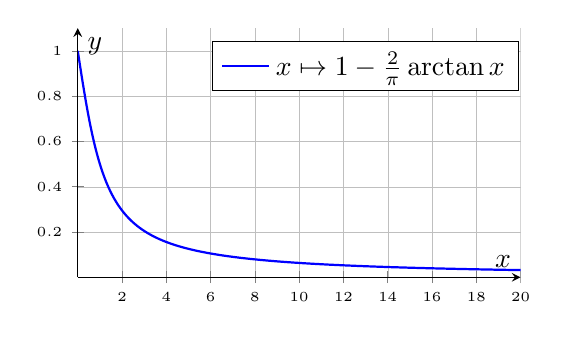
\begin{tikzpicture}
    \begin{axis}[
      width=160pt,
      height=90pt,
      compat=1.5.1,
      grid style={ultra thin},
      every axis plot post/.append style={thick},
      x tick label style={font=\tiny},
      y tick label style={font=\tiny},
      scale only axis,
      grid=major,
      axis lines=middle,
      xlabel={$x$},
      ylabel={$y$},
      xmin=0,
      xmax=20,
      domain=0:20,
      ymin=0,
      ymax=1.1,
      xtick={0,2,4,...,20},
      ytick={0,0.2,0.4,...,1},
      restrict y to domain=-20:20,
      legend style={at={(0.65,0.95)},anchor=north,nodes={right}},
    ]
      \addplot[mark=none,color=blue, samples=500]{1-(2/pi)*rad(atan(x))};
      \addlegendentry{$x \mapsto 1-\frac{2}{\pi}\arctan x $};
    \end{axis}
  \end{tikzpicture}

  \caption{
    Loss normalization function.
    \label{fig:arctan}
  }
\end{figure}


\subsection{Fighting Heterogeneity with Clustering\label{sec:radar.archi.cluster}}

The clustering algorithm seeks to gather similar participants together in more homogeneous sub-federations when appropriate. 
\textcite{nguyen_FLAMETamingBackdoors_2022} and~\textcite{ye_PFedSAPersonalizedFederated_2023} both measure participants' similarity by comparing the distance between model updates. 
This is biased, as models that are statically different might still produce relevant results. 
\thecontrib addresses this issue by defining similarity as the distance between participants emitted evaluations. 
Indeed, since all participants evaluate the same models, the variation in evaluation results reflects a difference in the evaluation datasets. 
Therefore, participants having similar datasets should issue similar evaluations. 

We note $\pdist$ the distance between the evaluations of $\p[i]$ and $\p[j]$ at round $r$.
$\pdist$ is defined as the cosine similarity between $\p[i]$ and $\p[j]$  issued evaluation vectors $\issue$ and $\issue[j]$, or $\delta(\issue,\issue[j])$.
We then iteratively group similar participants into different clusters, leveraging hierarchical clustering. 
Initially, each participant is assigned to a different cluster.
Then, each closest pair of clusters is merged, thus reducing the number of clusters.
The process is repeated until the distance between the two closest clusters exceeds a given threshold.
\Cref{fig:radar.clustering} illustrates this process.

\begin{figure}
    \centering
    \begin{tikzpicture}[]
	\node[leaf, c1] (a) {a};
	\node[leaf, c1, right of=a] (b) {b};
	\node[leaf, c1, right of=b] (c) {c};
	\node[leaf, c1, right of=c] (d) {d};
	\node[leaf, c1, right of=d] (e) {e};
	\node[leaf, c2, right of=e] (f) {f};
	\node[leaf, c2, right of=f] (g) {g};
	\node[leaf, c2, right of=g] (h) {h};
	\node[leaf, c3, right of=h] (i) {i};
	
	\node (ab) at ($(a)!0.5!(b)$) {};
	\node[above of=ab, node distance=0.4cm,label={[label distance=0, text=orange]175:0.1}] (ab1) {};
	
	\draw[c1] (a) |- (ab1.center);
	\draw[c1] (b) |- (ab1.center);
	
	\node (cd) at ($(c)!0.5!(d)$) {};
	\node[above of=cd, node distance=0.6cm,label={[label distance=
0, text=orange]175:0.3}] (cd1) {};
	
	\draw[c1] (c) |- (cd1.center);
	\draw[c1] (d) |- (cd1.center);
	
	\node (bc) at ($(b)!0.5!(c)$) {};
	\node[above of=bc, node distance=1.2cm,label={[label distance=
0.4cm, text=orange]175:0.7}] (bc2) {};
	
	\draw[c1] (ab1.center) |- (bc2.center);
	\draw[c1] (cd1.center) |- (bc2.center);
	
	\node (bce) at ($(bc2)!0.5!(e)$) {};
	\node[above of=bce, node distance=0.8cm,label={[label distance=
0.6cm, text=orange]175:0.8}] (bce3) {};
	\node[above of=bce3, node distance=0.6cm, label={[label distance=0cm, text=orange]-10:$C_k$}] (bce4) {};
	
	\draw[c1] (bc2.center) |- (bce3.center);
	\draw[c1] (e) |- (bce3.center);
	\draw[c1] (bce3.center) -- (bce4.center);
	
	\node (gh) at ($(g)!0.5!(h)$) {};
	\node[above of=gh, node distance=0.5cm,label={[label distance=0cm, text=violet]175:$0.2$}] (gh1) {};
	
	\draw[c2] (g) |- (gh1.center);
	\draw[c2] (h) |- (gh1.center);	
	
	\node (fgh) at ($(f)!0.5!(gh)$) {};
	\node[above of=fgh, node distance=0.95cm,label={[label distance=5, text=violet]175:0.6}] (fgh1) {};
	\node[above of=fgh1, node distance=1.1cm, label={[label distance=0cm, text=violet]-10:$C_\ell$}] (fgh2) {};

	\draw[c2] (f) |- (fgh1.center);
	\draw[c2] (gh1.center) |- (fgh1.center);
	\draw[c2] (fgh1.center) |- (fgh2.center);
	
	\node (bcefgh) at ($(bce4)!0.5!(fgh1)$) {};
	\node[above of=bcefgh, node distance=1cm,label={[label distance=0.9cm, text=black]175:1.2}] (bcefgh3) {};	
	
	\draw (bce4.center) |- (bcefgh3.center);
	\draw (fgh2.center) |- (bcefgh3.center);	
	
	\node (all) at ($(bcefgh3)!0.5!(i)$) {};
	\node[above of=all, node distance=1cm] (all1) {};
	\node[above of=i, node distance=2cm, label={[label distance=0cm, text=teal]-10:$C_i$}] (last1) {};
	\node[above of=all, node distance=1.5cm,label={[label distance=1.25cm, text=black]175:1.3}] (last2) {};	
	
	%\draw[c2] (all.center) -- (all1.center);
	\draw (bcefgh3.center) |- (last2.center);
	\draw[c3] (i) |- (last1.center);
	\draw (last1.center) |- (last2.center);	
	
	\node[left of=bce4, node distance=3cm, label={[label distance=-0.1cm,text=red]75:threshold = 1.0}] (threshold) {};
    \draw[thick, color=red,dash pattern={on 12pt off 3pt}] (last1.east) -- (threshold);
	
	\node[left of=a, node distance=0.5cm] (O) {};
	\node[above of=O, node distance=3cm] (arrow) {};
	\draw[->] (O) -- node[midway, sloped, above] {Cluster distance} (arrow);		
	
\end{tikzpicture}
    \caption{
      Hierarchical clustering process.
      \label{fig:radar.clustering}
    }
\end{figure}

While hierarchical clustering does not require the number of clusters as an input, choosing the right threshold can be challenging.
Contrarily to~\textcite{ye_PFedSAPersonalizedFederated_2023} who manually adjust this parameter on a per-dataset basis, \thecontrib leverages a dynamic threshold based on the mean inter-distance $\mdist$ between the clusters at round $r$.
This threshold $\theta$ is expressed as:
\begin{equation}\label{eq:mean_inter_cluster_distance}
    % \theta = \beta\mdist = \beta\sum_{\substack{k,\ell\in\C{},\\ k \ne l}}\frac{\kdist}{|\C{}|(|\C{}|-1)} 
    \theta = \beta\mdist = \frac{\beta}{|\C{}|(|\C{}|-1)}\sum_{\substack{k,\ell\in\C{},\\ k \ne l}}\kdist 
\end{equation}
where $\beta$ is a tunable hyperparameter, and $\kdist$ the distance between two clusters $\c$ and $\c[\ell]$, defined as the distance between their centroids: $\delta(\center,\center[\ell])$.
The centroid $\center$ of a cluster $\c$ is the average of the issued evaluations from its participants at round $r$, \ie, we have $\center = \frac{1}{|\c|}\sum_{i \in \c}\issue[i]$.

Based on the results of the clustering, the server can then aggregate the models of each cluster $\c$ separately, using the reputation system described in \Cref{sec:radar.archi.reput}.
Consequently, the server maintains as many global models $\wbar$ as there are clusters at each round. 
Note that this is another difference with \texttt{FLAME}~\cite{nguyen_FLAMETamingBackdoors_2022}, which only produces a single common model for every participant. 


\subsection{Ensuring Quality Contributions with Reputation\label{sec:radar.archi.reput}}

The reputation system centrally computes the weights $\weight, \forall \p \in \c$ used in the aggregation of each cluster model $\wbar$ at round $r$ (see \Cref{sec:radar.archi.xeval}).
Given the existence of methods for common tasks, such as contribution filtering, \thecontrib models trust using a multivalued Dirichlet probability distribution~\cite{fung_DirichletBasedTrustManagement_2011}. 
However, the evaluations $\rece[i]$ received by a participant $\p$ are continuous over $[0,1]$, and thus need to be discretized into a set of $q$ possible values $\mathcal{E} = \{\varepsilon_1, \varepsilon_2, \ldots, \varepsilon_q\}$. 

A Dirichlet distribution on the outcome of an unknown event (\ie, the mean of the received evaluation $\frac{1}{n}\sum_{\e \in \rece} \e$) is usually based on the combination of an initial belief vector and a series of cumulative observations~\cite{fung_DirichletBasedTrustManagement_2011}. 
As a complete cross evaluation is already available at the first round, \thecontrib does not require an initial belief vector to bootstrap reputation.

Following the notation used by~\textcite{fung_DirichletBasedTrustManagement_2011}, we note $\vec{\gamma}^r = \{\gamma_{1}^r,\gamma_{2}^r,\ldots,\gamma_{q}^r\}$ the cumulative evaluations received by $\p$: $\gamma_{2}^r=3$ means that three evaluations in $\rece$ had values bounded by $\left[\frac{1}{q},\frac{2}{q}\right[$.
We then note $\Prob = {\langle\prob[\varepsilon_1],\prob[\varepsilon_2], \ldots, \prob[\varepsilon_q]\rangle}$ the probability distribution vector for the received evaluation of a participant, where $\sum_{s=1}^{q}\prob[\varepsilon_s] = 1$.
Leveraging the cumulative evaluations $\vec{\gamma}^r$, the probability $\cond[\varepsilon_s]$ is given by $\cond[\varepsilon_s] = \gamma_{s} / \sum_{m=1}^{q}{\gamma_{m}}$.

The system further needs to limit the ability of potential malicious participants to manipulate their evaluations, either by badmouthing another participant, or by artificially raising their own ratings.
Consequently, the evaluations issued by a participant $\p \in \c$ are weighted according to their similarity with other cluster members'~\cite{xiong_PeerTrustsupportingreputationbased_2004} as $\e[i][j][\prime] = \e sim(\issue,\issue[\c])$, where the similarity is defined as:

\begin{equation}\label{eq:sim_reput}
  sim(\issue,\issue[\c]) = 1 - \sqrt{
    \frac{
      \sum_{j=1}^{n}{
        {\left(\e - \sum_{i \in \c} \frac{\e}{|\c|}\right)}^{2}
      }
    }
    {
      |\P|
    }
  }.
\end{equation}


To prevent attacks phased over multiple rounds, while preventing past mistakes from permanently impacting a participant, we use an exponential decay as forgetting factor, noted $\lambda \in [0,1]$. The reputation $\rep$ of a participant $\p$ at round $r$ based on the prior knowledge $\gamma^r_i$ of this participant is given by \Cref{eq:reputation_history}.
Note that a small $\lambda$ gives more importance to recent evaluations: $\lambda=0$ only considers the last round while $\lambda=1$, considers all round with equal weight.  
Based on $\rep$, the weight $\weight$ of $\w$ for aggregation in $\wbar$ (see Step~\ref{item:xeval.3} in~\Cref{sec:radar.archi.xeval}) is given by \Cref{eq:weight_computation}.

\begin{multicols}{2}
  \begin{equation}\label{eq:reputation_history}
    \rep = \sum_{\kappa=1}^{r}\lambda^{r-\kappa}\gamma_i^{\kappa}
  \end{equation}\break
  \begin{equation}\label{eq:weight_computation}
    \weight = \frac{\rep}{\sum_{j}^{|\c|}\rep[j]}
  \end{equation}
\end{multicols}

As such, the weight $\weight$ of $\p$ will be proportional to its reputation, and therefore the evaluations it received over time.
The attackers' evaluations only vary on the subset of samples that are impacted. 
Consequently, the differences between their reputation scores and those of legitimate participants can be relatively small, despite remaining meaningful. 
We apply a sigmoid function to convert these scores to aggregation weighs and accentuate this difference.
This sigmoid function is the normal distribution cumulative density function adjusted with the $\sigma$ parameter.
